\setchapterstyle{kao}
\setchapterpreamble[u]{\margintoc}

\chapter{The IceCube Neutrino Observatory}
\labch{icecube}

\todo{(Re-)write IceCube chapter for PhD thesis (just copy paste from M.Sc.).}

This chapter explains the detection principle of the IceCube Neutrino Observatory as well as one of the reconstruction algorithms applied to extract information from the raw detector signals.
Section \ref{sec:icecube_array} first presents the layout of IceCube and DeepCore before Section \refsec{cherenkov_effect} and \ref{sec:energy_loss} explain the Cherenkov effect and the propagation of particles through ice.
Finally, Section \refsec{event_reconstruction} outlines the reconstruction algorithm itself in detail.

\section{The IceCube In-Ice Array} \labsec{icecube_array}

\begin{figure}[ht]
	\centering
    \subfloat[IceCube Neutrino Observatory][Schematic sketch]{ \labfig{icecube_array}
    \includegraphics[width=0.55\linewidth]{figures/icecube_deepcore/IceCubeArray_slim.png}
    }
    \subfloat[Digital Optical Module (DOM)][Design and components of a DOM]{ \labfig{DOM_design}
    \includegraphics[width=0.4\linewidth]{figures/icecube_deepcore/DOM_schematic.png}
    }
	\caption[IceCube Neutrino Observatory and Digital Optical Module]{The IceCube Neutrino Observatory and a schematic view of the Digital Optical Module (DOM). More detailed information can be found in \cite{2017JInst..12P3012A_Instrumentation_Systems}.}
\end{figure}

The IceCube Neutrino Observatory \sidecite{2017JInst..12P3012A_Instrumentation_Systems} is a cubic-kilometer particle detector located at the geographic south pole.
The detector consists of 86 vertical strings with 5160 optical sensors called digital optical modules (DOMs) \sidecite{ABBASI2009294_data_acquisition}.
Figure \ref{fig:icecube_array} shows a schematic overview of the detector layout with its main components.
The strings were drilled down into the Antarctic ice in a hexagonal arrangement shown in Figure \reffig{icecube_top_view}.
60 optical sensors are placed on each string at depths of 1450-2450\,m below the ice.
IceCube is designed to detect neutrinos in the energy range $\mathcal{O}$(GeV)-$\mathcal{O}$(PeV).
Neutrinos can only be detected by the secondary charged particles created when they interact in the ice.
The optical sensors detect Cherenkov light produced by these charged particles (see Section \refsec{cherenkov_effect}).
Using the observed light pattern, the neutrino energy, direction, and flavor can be reconstructed as described in Section \refsec{event_reconstruction}.
The DOMs are made of a spherical glass housing containing a 10\," photomultiplier tube (PMT) in addition to the readout and processing electronics.
The modules are made to collect light, digitize the resulting PMT signal and send the data to the central data acquisition at the surface if a trigger condition is met.
The design of a DOM and its components is shown in Figure \reffig{DOM_design}.

\begin{figure}[h]
    \begin{center}
        \includegraphics[trim={2.0cm, 1.5cm, 0, 0}, clip, width=0.65\linewidth]{figures/icecube_deepcore/icecube_top_view_bw.pdf}
    \end{center}
    \caption[IceCube top view]{Top view of the IceCube array.}
    \labfig{icecube_top_view}
\end{figure}

The main part of IceCube is formed by 78 strings with 125\,m horizontal spacing and 17\,m vertical spacing between DOMs.
This results in a neutrino detection energy threshold of 100\,GeV. There are 8 additional strings that form a denser sub-array of IceCube called DeepCore \sidecite{DeepCore_design_Abbasi2012615}.
DeepCore is at the bottom-center of the detector and includes these 8 strings as well as the 7 surrounding IceCube strings in the fiducial volume shown in Figure \reffig{icecube_top_view}.
The strings in this volume have an average distance of about 70\,m.
The majority of the DeepCore DOMs are placed between 2100\,m and 2450\,m below the ice and the vertical spacing is 7\,m.
Around 2050\,m there is a dust layer with bad optical properties. Above the dust layer, there are a few additional DeepCore modules used as a veto cap.
The denser spacing and the application of high quantum efficiency DOMs in DeepCore as well as the fact that the ice between 2100\,m and 2450\,m has the best optical properties leads to a lowered neutrino detection energy threshold of around 5\,GeV.
DeepCore is optimized for the observation of neutrinos in the energy range of $10-100$\,GeV.
This is the energy range where the oscillation signal from atmospheric neutrinos can be observed and studied.
The surrounding IceCube strings and the veto cap are used to reject atmospheric muons that are the main background in neutrino oscillation measurements.

The coordinate system \sidecite{2017JInst..12P3012A_Instrumentation_Systems} used in IceCube is centered at 46500'E, 52200'N at an elevation of 883.9\,m.
It is defined as a right-handed coordinate system with the y-axis pointing along the Prime Meridian (Grid North) towards Greenwich, UK and the x-axis pointing 90\,degrees clockwise from the y-axis (Grid East).
The z-axis is normal to the  Earth's surface, pointing away from the surface.
Additionally, the depth in IceCube is defined as the vertical distance from the ice surface, set to be at an elevation of 2832\,m.


\subsection{In-Ice Array}

\subsubsection{DeepCore}

\subsection{IceTop}

\subsection{Digital Optical Modules}


\section{Propagation of Particles in Ice}

When charged particles travel through matter they interact and lose energy by several interaction processes.
The Cherenkov light emitted by the particles as described in Section \refsec{cherenkov_effect} only contributes a small amount to the total energy loss.
The dominant processes depend on the type of Cherenkov light source, which we can broadly categorize into the three groups: quasi-continuous energy loss by muons, electromagnetic cascades, and hadronic cascades.

\paragraph{Muons} lose their energy mainly by \textit{ionization}, \textit{bremsstrahlung}, \textit{pair production} and the \textit{photo-nuclear interaction}.
Considering that ionization only has a weak energy dependence for muons above 1\,GeV and combining the other three components into one, the total energy loss is given by
\begin{equation}
    -\frac{\mathrm{d}E}{\mathrm{d}x} = a_I(E) + b_R(E) \cdot E,
    \labeq{radiative_losses}
\end{equation}
where $E$ is the energy and $a_I(E)$ and $b_R(E) \cdot E$ are the energy loss by ionization and the combined radiative losses, respectively.
For the energy range of interest for this work, the parameters $a_I(E)$ and $b_R(E)$ only have a weak energy dependence and equation \refeq{radiative_losses} reduces to
\begin{equation}
    -\frac{\mathrm{d}E}{\mathrm{d}x} = a + b \cdot E.
    \labeq{radiative_losses_simple}
\end{equation}
This description results in a critical energy $E_{crit}=a/b$ separating the two energy regimes where ionization or radiative losses are dominant.
Typical values are $a \approx 2.59$\,MeV/cm and $b \approx 3.63 \cdot 10^{-6}$\,cm$^{-1}$ \cite{2004hep.ph....7075C} leading to a critical energy of $\sim 770$\,GeV.
Since the considered energy range for atmospheric neutrino oscillations is below the critical energy we only consider ionization losses by setting $b=0$ which easily relates the range of a muon $R_\mu$ to its initial energy by
\begin{equation}
    R = \frac{E_0}{a}.
    \labeq{muon_range_approx}
\end{equation}
With equation \refeq{muon_range_approx} it is clear that by measuring the length of a muon track, its energy can be estimated if the full track is contained in IceCube.
This treatment is only an approximation and does not take into account the stochastic nature of some of the energy losses.
Especially bremsstrahlung and photo-nuclear interactions occur rarely, but when they happen, they deposit a large amount of energy. More detailed information is found in \sidecite{LRaedel}.


\subsection{Cherenkov Effect} \labsec{cherenkov_effect}

Cherenkov radiation is emitted when a charged particle moves through a medium with a velocity that is greater than the speed of light in that medium.
The continuous energy loss due to the emission of Cherenkov radiation is small, at the order of $\mathcal{O}$($10^{-4}$), as compared to the main energy losses that will be described in Section \refsec{energy_loss}.
The observation of this radiation in IceCube and DeepCore, however, is fundamental for the detection of the charged particles originating from the neutrino interactions that were outlined in Section \refsec{neutrino_interactions}.
The Cherenkov effect was first observed by Pavel Cherenkov in 1934 \sidecite{CherenkovPhysRev.52.378}.
As can be derived from trigonometry, the Cherenkov light is emitted in a parallel wavefront at the Cherenkov angle
\begin{equation}
    \theta_c = \arccos\Big(\frac{1}{\beta n}\Big),
    \labeq{cherenkov_angle}
\end{equation}
with $n$ being the refractive index of the medium and $\beta$ the speed of the particle in units of the speed of light.
A sketch of the wavefront is shown in Figure \reffig{cherenkov_light_front}, where the black circles depict spherically emitted light and the blue line is the formed Cherenkov light front.
\begin{figure}[h]
    \centering
    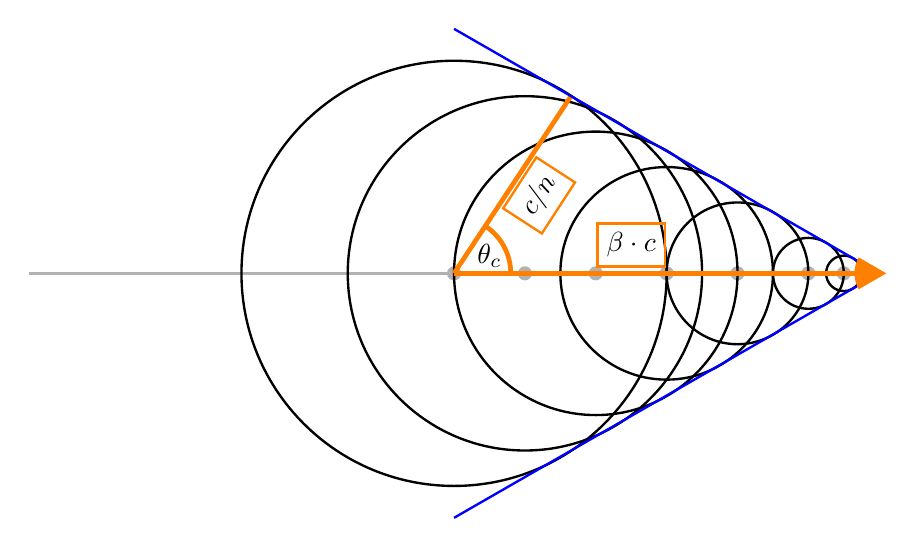
\begin{tikzpicture}[scale=0.9]
        \draw[draw=none,fill=gray!60] (8,0) circle (0.1);
        \draw[draw=none,fill=gray!60] (9,0) circle (0.1);
        \draw[draw=none,fill=gray!60] (10,0) circle (0.1);
        \draw[draw=none,fill=gray!60] (11,0) circle (0.1);
        \draw[draw=none,fill=gray!60] (12,0) circle (0.1);
        \draw[draw=none,fill=gray!60] (13,0) circle (0.1);
        \draw[draw=none,fill=gray!60] (13.5,0) circle (0.1);
        
        \draw[line width=0.3mm, gray!60] (2,0)--(14,0);
        
        \draw[line width=0.3mm] (8,0) circle (3);
        \draw[line width=0.3mm] (9,0) circle (2.5);
        \draw[line width=0.3mm] (10,0) circle (2);
        \draw[line width=0.3mm] (11,0) circle (1.5);
        \draw[line width=0.3mm] (12,0) circle (1);
        \draw[line width=0.3mm] (13,0) circle (0.5);
        \draw[line width=0.3mm] (13.5,0) circle (0.25);
        
        \draw[orange, line width=0.6mm] (8,0)--(14,0);
        \draw[orange, line width=0.6mm] (8,0)--(9.65,2.5);
        
        \draw[orange, line width=0.6mm] (8.8,0) arc (0:55:0.8cm);
        
        \draw[blue, line width=0.3mm] (8,3.45) -- (14,0);
        \draw[blue, line width=0.3mm] (8,-3.45) -- (14,0);
        
        \draw[draw=none,fill=orange] (14.1,0)-- +(210:0.45cm)arc (210:150:0.45cm) -- cycle;
        
        \node[] at (8.5,0.25) {$\theta_c$};

        \node[draw=orange,line width=0.3mm] at (10.5,0.4) {$\beta \cdot c$};
        \node[draw=orange,line width=0.3mm,, rotate=57] at (9.2,1.1) {$c/n$};
    \end{tikzpicture}
    \caption[Cherenkov light front]{Schematic formation of the Cherenkov light front (blue) produced by a charged particle traveling faster than the speed of light in the medium. The black circles are spherically emitted light and the orange arrow shows the direction of the particle.}
    \labfig{cherenkov_light_front}
\end{figure}
Typical values for the Antarctic ice are $n \approx 1.3$ and as a result $\theta_c \approx 41^\circ$ \sidecite{SEuler}.
Additionally, one can calculate the number of photons produced by a Cherenkov emitter based on the description in \sidecite{Frank_Tamm}.
For a wavelength $\lambda$ with (300\,nm < $\lambda$ < 500\,nm) 250 photons per cm are emitted assuming a very relativistic particle with $\beta \simeq 1$ \sidecite{raedel_wiebusch_cherenkov_yield}.


\subsection{Energy Losses} \labsec{energy_loss}


\subsubsection{Muons}


\subsubsection{Electromagnetic Showers}

Electromagnetic cascades are induced by electrons and positrons or photons.
All of them are either produced directly in the neutrino interactions or in interactions of secondary particles.
Photons lose energy via pair production whereas for electrons and positrons the dominant energy loss is due to bremsstrahlung.
For both cases, the interaction process happens repeatedly and an electromagnetic shower is formed when pair production and bremsstrahlung take place in turn.
Every time one of the interactions takes place, more electrons and positrons or photons are produced with smaller energy. 
This proceeds until the energy of the particles falls below the critical energy $E_c$ and the remaining energy is quickly lost.
For electrons and positrons, this happens through ionization and excitation of the surrounding atoms.
For photons, the Compton effect and the photoelectric effect become the dominant energy losses.
Electromagnetic showers are characterized by the radiation length $X_0$ at which the energy of electrons or positrons is reduced to $1/e$ of their initial energy.
For photons, $X_0$ is $7/9$ of the mean free path for pair production. For ice, the critical energy is $E_c \approx 78$\,MeV and the radiation length is $X_0 \approx 39.3$\,cm \sidecite{PhysRevD.98.030001}.


\subsubsection{Hadronic Showers}

Hadronic cascades are always produced in the neutrino interactions described in Section \refsec{neutrino_interactions}, either from the breaking nucleus or as decay products.
Similar to an electromagnetic cascade, a hadronic cascade forms as a result of the production of secondary particles from the strong interactions of hadrons with the traversed matter.
Hadronic cascades also contain an electromagnetic component, for example through the decay of neutral pions into two photons. 
The shower profile and the light emission are very dependent on the produced particle type, which leads to larger fluctuations between individual showers with the same energy.
The observed energy also varies, because energy gets lost in the hadronic binding process and muons and neutral particles produce less light and no light, respectively.
On top of that, hadrons have a higher energy threshold for Cherenkov light production, due to their higher mass.
The relative brightness of hadronic showers as compared to electromagnetic showers is given by \sidecite{LRaedel}
\begin{equation}
    F(E) = \frac{T_\mathrm{hadron}}{T_\mathrm{EM}},% = 1 - (1 - f_0)\Big(\frac{E}{E_s}\Big)^{-m}
    \labeq{relative_shower_brighness}
\end{equation}
where $T_\mathrm{hadron/EM}$ is the total track length of a hadronic/electromagnetic shower with the same energy.
The ratio $F(E)$ is always smaller than 1, but increases with energy as the electromagnetic fraction of the hadronic cascade becomes larger.
A more detailed parameterization of $F(E)$, as well as fitted values for several particle types, can be found in \sidecite{LRaedel}.


\section{Particle Signatures in IceCube}

\subsection{Neutrinos}

\subsection{Atmospheric muons}
